\documentclass[aspectratio=1610]{beamer}
\usepackage{graphicx}
\usetheme{Madrid}
\usepackage{tikz}
\usetikzlibrary{automata, positioning, arrows}
\tikzset{
->, % makes the edges directed
>=stealth, % makes the arrow heads bold
node distance=2.5cm, % specifies the minimum distance between two nodes. Change if necessary.
every state/.style={thick, fill=gray!10}, % sets the properties for each ’state’ node
initial text=$ $, % sets the text that appears on the start arrow
}
\title[Dynamic Logic for Symbolic Execution]{A Dynamic Logic for Symbolic Execution for the Smart Contract Programming Language Michelson}
\author[Arvay, Doan, Thiemann]{Barnabas Arvay, Thi Thu Ha Doan, \underline{Peter Thiemann}}
\institute[]{University of Freiburg}
\date{September 18, 2024 (ECOOP)}


\begin{document}
\begin{frame}
  \titlepage
\end{frame}

\begin{frame}
  \frametitle{Smart Contracts}
  \begin{itemize}
  \item Code running on a blockchain
  \item Code is public; open to scrutiny
  \item Smart contract vulnerabilities have been responsible for financial losses measuring over \$12.3 billion.\footnote{
      [Chu et al: A survey on smart contract vulnerabilities: Data sources, detection and repair]}
  \item Code is immutable; impossible to amend
  \item[$\Rightarrow$] Verification of smart contracts is required!
  \end{itemize}
\end{frame}
\begin{frame}
  \frametitle{Context of our work}
  \begin{block}<+->{Interest}
  \begin{itemize}
  \item Automatic verification
  \item Functional specification
    \begin{itemize}
    \item Pre-/postconditions
    \item Contract life cycle
    \end{itemize}
  \end{itemize}
\end{block}
\begin{block}<+->{Methods}
  \begin{itemize}
  \item Symbolic execution
  \end{itemize}
\end{block}
\begin{block}<+->{Domain}
  \begin{itemize}
  \item Michelson (Tezos blockchain)
  \end{itemize}
\end{block}
\end{frame}
\begin{frame}
  \frametitle{Michelson --- language of the Tezos blockchain}
  \begin{block}<+->{Features}
  \begin{itemize}
  \item Purely functional
  \item Simply typed
  \item Stack-based
  \item Usual datatypes $+$ blockchain specific (tokens, operations, elliptic curves, \dots)
  \end{itemize}
\end{block}
\begin{exampleblock}<+->{Typing and execution}
  \begin{itemize}
  \item Execution \hspace{1ex}\includegraphics[scale=0.65]{add-semantics}
  \item Typing\qquad \includegraphics[scale=0.65]{add-typing}
  \item Program typing
    \begin{displaymath}
      \frac{p :: A \Rightarrow B \quad q :: B \Rightarrow C}{(p;q) :: A \Rightarrow C}
    \end{displaymath}
  \end{itemize}
\end{exampleblock}
\end{frame}
\begin{frame}[fragile]
  \frametitle{Michelson --- Semantics}
\begin{block}<+->{Typing of a contract}
  \Large\vspace{-\baselineskip}
  \begin{displaymath}
    (\mathit{param} \times \mathit{input\text{-}store}) : [] \quad\Rightarrow\quad
    (\mathit{list~operation} \times \mathit{output\text{-}store}) : []
  \end{displaymath}
\end{block}
\begin{exampleblock}<+->{Code example}
\begin{verbatim}
CAR; UNPAIR; ADD; NIL operation; PAIR
\end{verbatim}
\end{exampleblock}
\begin{block}<+->{Inter-transaction semantics}
  \begin{itemize}
  \item No direct contract calls
  \item Instead:
    \begin{itemize}
    \item \textit{operation} can be a contract call
    \item runtime system executes the list of operations
    \item runtime system maintains transactional semantics
    \end{itemize}
  \end{itemize}
\end{block}
\end{frame}
\begin{frame}
  \frametitle{Michelson --- Illustrated inter-transaction semantics}
  \begin{itemize}[<+->]
  \item start transaction \hfill pending [run A]
  \item run A\phantom{2} \qquad returns \qquad{} [run B, run C] \hfill pending [run B, run C]
  \item run B\phantom{2} \qquad returns \qquad{} [run B1, run B2] \hfill pending [run B1, run B2, run C]
  \item run B1 \qquad returns \qquad{} []  \hfill pending [run B2, run C]
  \item run B2 \qquad returns \qquad{} []  \hfill pending [run C]
  \item run C\phantom{2} \qquad returns \qquad{} []  \hfill pending []
  \item transaction complete
  \end{itemize}
  
\end{frame}
\begin{frame}
  \frametitle{Symbolic execution using dynamic logic}
  \begin{block}<+->{Dynamic Logic (DL)}
  \begin{itemize}
  \item Modal logic for reasoning about programs [Pratt'76, Harel, Kozen, Tiuryn 2002]
  \item Propositional logic $+$ modalities $[p]$ and $\langle p\rangle$ \hfill ($p$ a program fragment)
  \item $[p]\Psi$ states \emph{partial correctness}\hfill (all we need here)
  \item Key properties of the modality
    \begin{enumerate}
    \item $[p;q]\Psi \leftrightarrow [p][q]\Psi$
    \item $[\mathtt{if}~\Phi~p~q]\Psi \leftrightarrow (\Phi \to [p]\Psi) \vee (\neg\Phi \to [q]\Psi)$
  \end{enumerate}
  \end{itemize}
\end{block}
\begin{block}<+->{Symbolic Execution (SE)}
  \begin{itemize}
  \item Running a program on symbolic values
  \item Insights on key properties (by the KeY people)
    \begin{enumerate}
    \item $[i]\Psi$ specifies SE for single instructions $i$
    \item Generates path formulas for SE
  \end{enumerate}
  \end{itemize}
\end{block}
\end{frame}
\begin{frame}
  \frametitle{Contents of paper}
  \framesubtitle{Mechanized in Agda; focus on simplicity}
  \begin{itemize}
  \item Intrinsically-typed representation of Michelson programs
  \item Parameterized semantics (concrete and abstract execution)
    \begin{itemize}
    \item small step / partial function
    \item (required transformation from big-step to small-step)
    \end{itemize}
  \item Formalized (part of) the runtime system for inter-transaction semantics
  \item Semantics of the DL / abstract semantics
  \item Soundness of the DL
    \begin{itemize}
    \item family of abstraction relations (values, stacks, execution states, \dots)
    \item splitting of abstract states
  \end{itemize}
  \end{itemize}
\end{frame}
\begin{frame}
  \frametitle{Soundness illustrated}
  \begin{center}
  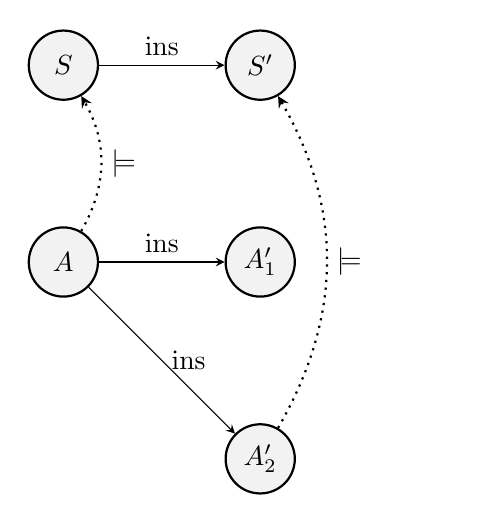
\begin{tikzpicture}
    \node[state] (q1) {$S$};
    \node<3->[state, right of=q1] (q2) {$S'$};
    \node<1->[state, below of=q1] (a0) {$A$};
    \node<2->[state, right of=a0] (a1) {$A_1'$};
    \node<2->[state, below of=a1] (a2) {$A_2'$};
    \node [below of=a0] (x0) {};
    \node [right of=q1] (x1) {};
    \node [right of=x1] (x2) {};
    \draw<3-> (q1) edge[above] node{ins} (q2);
    \draw<1-> (a0) edge[dotted, thick, right, bend right] node {$\models$} (q1);
    \draw<4-> (a2) edge[dotted, thick, right, bend right] node {$\models$} (q2);
    \draw<2-> (a0) edge[above] node{ins} (a1)
              (a0) edge[right] node{ins} (a2);
  \end{tikzpicture}
\end{center}
\end{frame}
\begin{frame}
  \frametitle{A glimpse on parameterized semantics}
  \begin{flushleft}
    \includegraphics[scale=0.5]{Contract}
    \\
    \includegraphics[scale=0.5]{Blockchain}
  \end{flushleft}
\end{frame}
\begin{frame}
  \frametitle{A glimpse on abstract values}
  \begin{block}<+->{Representation of an abstract value}
    \begin{itemize}
    \item Typed symbolic variable
    \item Set of typed equality constraints \quad $x = t$ \quad (variable = term)
    \item Terms are variables, constants, or operators (i.e., Michelson instructions) applied to variables
    \end{itemize}
  \end{block}
  \begin{block}<+->{Consequences}
    \begin{itemize}
    \item Simplifies soundness proof
    \item Implementation: map constants and operators to SMT solver
    \end{itemize}
  \end{block}
  % \begin{block}<+->{Footnote}
  %   \begin{itemize}
  %   \item In paper: some extra constraints for comparing tokens
  %   \item Can be elided with most recent version of Michelson
  %   \end{itemize}
  % \end{block}
\end{frame}
\begin{frame}
  \frametitle{Related work}
  \begin{block}{DL for symbolic execution}
    \begin{itemize}
    \item SE for Java [KeY people - see Key book]
    \item Abstract execution [Steinh\"{o}fel, H\"{a}hnle]
    \end{itemize}
  \end{block}
  \begin{block}{Verification for Michelson}
    \begin{itemize}
    \item Mi-cho-Coq [Bernardo et al]: framework for the interactive proof assistant Coq
    \item Helmholtz [Nishida et al]: verifier based on refinement typing
    \item Abstraction interpretation [Bau et al]: MOPSA framework
    \end{itemize}
  \end{block}
\end{frame}
\begin{frame}
  \frametitle{Conclusions and future work}
  \begin{block}{Conclusions}
  \begin{itemize}
  \item Specification of symbolic execution for Michelson based on DL
  \item Includes inter-transaction semantics
  \item Soundness proof of the DL
  \item Basis for our implementation (see paper at APLAS'24 [Doan, Thiemann])\\
    which has found issues in two financial contracts deployed on the blockchain
  \end{itemize}
\end{block}
  \begin{block}{Future work}
    Towards a verified implementation: \\
    Close the gap between specification and implementation \\
    (e.g., handling loops on unknown values, interface to SMT solver)
  \end{block}
\end{frame}
\end{document}
